\title{Assignment 2: CS 215}
\author{Akash Trehan-150050031, Bhavya Bahl-150050110}

\documentclass[11pt]{article}

\usepackage{amsmath}
\usepackage{amssymb}
\usepackage{hyperref}
\usepackage{ulem}
\usepackage{graphicx}
\usepackage[margin=0.5in]{geometry}
\delimitershortfall-1sp
\newcommand\abs[1]{\left|#1\right|}
\usepackage{fancyhdr}
 
\pagestyle{fancy}
\fancyhf{}
\lhead{Akash Trehan-150050031, Bhavya Bahl-150050110}
\begin{document}
\maketitle

Ans 1.\begin{center}
$$Z=XY$$
We know that $f_Z(z) = \frac{\text{d}}{\text{d}z}(F_Z(z))$
$$F_Z(z) =P(XY \le z)= \int_{0}^{\infty}\int_{-\infty}^{\frac{z}{x}}f_{XY}(x,y)dydx + \int_{-\infty}^{0}\int_{\frac{z}{x}}^{\infty}f_{XY}(x,y)dydx$$
$$\implies f_Z(z)=\frac{\text{d}}{\text{d}z}(F_Z(z))=\frac{\text{d}}{\text{d}z}(\int_{0}^{\infty}\int_{-\infty}^{\frac{z}{x}}f_{XY}(x,y)dydx)+\frac{\text{d}}{\text{d}z}(\int_{-\infty}^{0}\int_{\frac{z}{x}}^{\infty}f_{XY}(x,y)dydx)$$
$$=\int_{0}^{\infty}\frac{\text{d}}{\text{d}z}(\int_{-\infty}^{\frac{z}{x}}f_{XY}(x,y)dy)dx+\int_{-\infty}^{0}\frac{\text{d}}{\text{d}z}(\int_{\frac{z}{x}}^{\infty}f_{XY}(x,y)dy)dx$$
$$=\int_{0}^{\infty}\frac{f_{XY}(x,\frac{z}{x}}{x}dx + \int_{-\infty}^{0}(-1)\frac{f_{XY}(x,\frac{z}{x}}{x}dx$$
$$Now\ P(X \le Y) = \int_{-\infty}^{\infty}\int_{x}^{\infty}f_{XY}(x,y)dydx$$
If X and Y are independent
$$P(X \le Y) = \int_{-\infty}^{\infty}f_X(x)(\int_{x}^{\infty}f_Y(y)dy)dx$$
$$=\int_{-\infty}^{\infty}f_X(x)(\int_{-\infty}^{\infty}f_Y(y)dy-\int_{-\infty}^{x}f_Y(y)dy)dx$$
$$=\int_{-\infty}^{\infty}f_X(x)(1-F_Y(x))dx$$
\newline
\newline
\end{center}

Ans 2.\begin{center}
$$Y_1=max(X_1,X_2,....,X_n)\ and\ Y_2=min(X_1,X_2,....,X_n)$$
Since $X_1,X_2,...,X_n$ are identically distributed, their cdf($=F_X(x)$) and pdf($=f_X(x) = F_X'(x)$)
$$P(X_i \le x) = F_X(x) \forall i in [1,n]$$
$$For\ Y_1 \le x,\ each\ of\ X_1,X_2,....,X_n \le x,$$
$$Thus\ P(Y_1\le x) = P(X_1\le x,X_2\le x,....,X_n \le x)$$
Since $X_1,X_2,....,X_n$ are independent,
$$cdf\ of\ Y_1 = F_{Y_1}(x) = P(Y_1 \le x) = P(X_1 \le x)P(X_2 \le x).....P(X_n \le x)$$
$$=(F_X(x))^n$$
$$pdf\ of\ Y_1 = F_{Y_1}'(x) = ((F_X(x))^n)' = n(F_X(x))^{n-1}F_X'(x)$$
\linebreak
$$Now\ P(X_i > x) = 1 - P(X_i \le x) = 1 - F_X(x)\ \forall i\ in\ [1,n]$$
$$For\ Y_2 > x,\ each\ of\ X_1,X_2,....,X_n > x,$$
$$Thus\ P(Y_2 > x) = P(X_1> x,X_2> x,....,X_n > x)$$
Since $X_1,X_2,....,X_n$ are independent,
$$P(Y_2 > x) = P(X_1 > x)P(X_2 > x).....P(X_n > x)$$
$$=(1 - F_X(x))^n$$
$$P(Y_2 > x) = 1 - P(Y_2 \le x) =(1 - F_X(x))^n$$
$$cdf\ of\ Y_2 = F_{Y_2}(x)=P(Y_2 \le x) = 1 - (1 - F_X(x))^n$$
$$pdf\ of\ Y_2 = F_{Y_2}'(x) = ((1 - F_X(x))^n)' = n(1 - F_X(x))^{n-1}F_X'(x)$$
\newline
\newline
\end{center}

Ans 3.\begin{center}
Since the total amount doubles in each trial, the amount bet in the $n^{th}$ trial = $2^{n-1}x$\linebreak
Amount won in the $n^{th}$ trial = $2^{n-1}x$
Total amount lost in the previous n-1 trials = $\sum\limits_{i=1}^{n-1}2^{i-1}x$
Net amount won = $2^{n-1}x-\sum\limits_{i=1}^{n-1}2^{i-1}x$
$$=2^{n-1}x-\frac{2^{n-1}-1}{2-1}x$$
$$=2^{n-1}x - (2^{n-1}-1)x$$
$$=x$$
\newline
\newline
\end{center}

Ans 4.\begin{center}
$$Covariance = E((x-\mu_x)(y-\mu_y))$$
$$=E(XY - X\mu_y - Y\mu_X + \mu_x\mu_y)$$
$$=E(XY) - \mu_yE(X) - \mu_xE(Y) + \mu_x\mu_y(\because\ E()\ is\ a\ linear\ operator.)$$
$$=E(XY) - \mu_y\mu_x - \mu_x\mu_y + \mu_x\mu_y$$
$$=E(XY) - \mu_x\mu_y$$
$$=E(XY) - E(X)E(Y)$$

$$E(XY) = \int_{-\infty}^{\infty}\int_{-\infty}^{\infty}xyf_XY(x,y)dxdy$$
If X and Y are independent $f_XY(x,y) = f_X(x)f_Y(y)$
$$E(XY) = \int_{-\infty}^{\infty}\int_{-\infty}^{\infty}xyf_XY(x,y)dxdy = \int_{-\infty}^{\infty}\int_{-\infty}^{\infty}xyf_X(x)f_Y(y)dxdy$$
$$=\int_{-\infty}^{\infty}xf_X(x)dx\int_{-\infty}^{\infty}yf_Y(y)dy$$
$$=E(X)E(Y)$$
$$\implies E(XY) - E(X)E(Y) = 0$$

Thus independence implies Covariance is 0.
But the converse may not always be true.

\textbf{Counter Example:}
Consider the set {1,2,3} with equal probability of selecting any one of the elements.

Now we select one element from the set.

Consider the random variables $X_1,X_2$ such that,
\[
X_1 = 
   \begin{cases} 
      1 &  Selected\ number\ is\ even\\
      0 & Selected\ number\ is\ odd 
   \end{cases}
\]

$X_2$ = Selected number

$$Now\ E(X_1)=1*\frac{1}{3} + 0*\frac{2}{3}=\frac{1}{3}$$
$$E(X_2)=1*\frac{1}{3}+2*\frac{1}{3}+3*\frac{1}{3}=2$$
$$E(X_1X_2) = 1*2*\frac{1}{3} + 0=\frac{2}{3} = E(X_1)E(X_2)$$
Hence Covariance of $X_1, X_2$ is 0.

Now when $X_2=1,\ then X_1 must be 0$(since 1 is odd). Hence,
$$P(X_1=1, X_2=1) = 0$$
$$But\ P(X_1=1) = 1*\frac{1}{3}\ and\ P(X_2=1)=\frac{1}{3}$$
$$Thus\  P(X_1=1, X_2=1) \neq P(X_1=1)P(X_2=1)$$
Hence $X_1\ and\ X_2$ are not independent.
Thus $Covariance = 0 \not \Rightarrow Independence$

\end{center}

Ans 5.\begin{center}
$$Var(X) = E((x-\mu)^2)$$
$$We\ know\ that\ E((x-c)^2)\ is\ minimum\ when\ c = \mu$$
$$Let c = \frac{a+b}{2}$$
$$Thus\ Var(X) \le E((x-\frac{a+b}{2})^2)$$
$$=\int_{a}^{b}(x - \frac{a+b}{2})^2 f_X(x) dx$$
$\frac{a+b}{2}$ is the mid-point of the interval [a,b].
Now to maximise $(x - \frac{a+b}{2})^2$ we need to take the value farthest from $\frac{a+b}{2}$ in the interval [a,b]. These values are x=a and x=b which give
$$(x - \frac{a+b}{2})^2 = (a - \frac{a+b}{2})^2 = (b - \frac{a+b}{2})^2 = (\frac{b-a}{2})^2$$
$$Hence \int_{a}^{b}(x - \frac{a+b}{2})^2 f_X(x) dx \le (\frac{b-a}{2})^2 \int_{a}^{b} f_X(x) dx$$
$=(\frac{b-a}{2})^2\ (\because$ the total probability over the entire range in 1)
$$Hence\ Var(X) \le (\frac{b-a}{2})^2=\frac{(b-a)^2}{4}$$
\newline
\newline
\end{center}

Ans 6.\begin{center}
The equation of tangent at $x=x_o$ is
$$\frac{y-g(x_o)}{x-x_o} = g'(x)$$
$$\implies y=(x-x_o)g'(x_o)+g(x_o)$$
As g(x) is a convex function
$$g(x) \ge y=(x-x_o)g'(x_o)+g(x_o)$$
$$\implies g(x) \ge (x-x_o)g'(x_o) + g(x_o)$$
$$\implies \int_{-\infty}^{\infty}g(x)f_X(x)dx \ge \int_{-\infty}^{\infty}((x-x_o)g'(x_o) + g(x_o))f_X(x)dx$$
$$E(g(x)) \ge (E(x) - x_o)g'(x_o) + g(x_o)$$
This holds for all $x=x_o$
Let $x_o=E(x)$
$$E(g(x)) \ge g(E(x))$$
Hence proved.
\newline
\newline
\end{center}
\pagebreak

Ans 7.\begin{center}
\begin{table}[h]
\centering
\begin{tabular}{llll}
                        & \textbf{Corr. Coeff.} & \textbf{QMI} & \textbf{Measure (3)} \\
\textbf{Normal Case}    & 0.9844                      & 0.0359       & 1.4735               \\
\textbf{Scrambled case} & 0.0029                      & 2.5222e-06   & 0.0242              
\end{tabular}
\end{table}
\end{center}

\begin{figure}[h]
  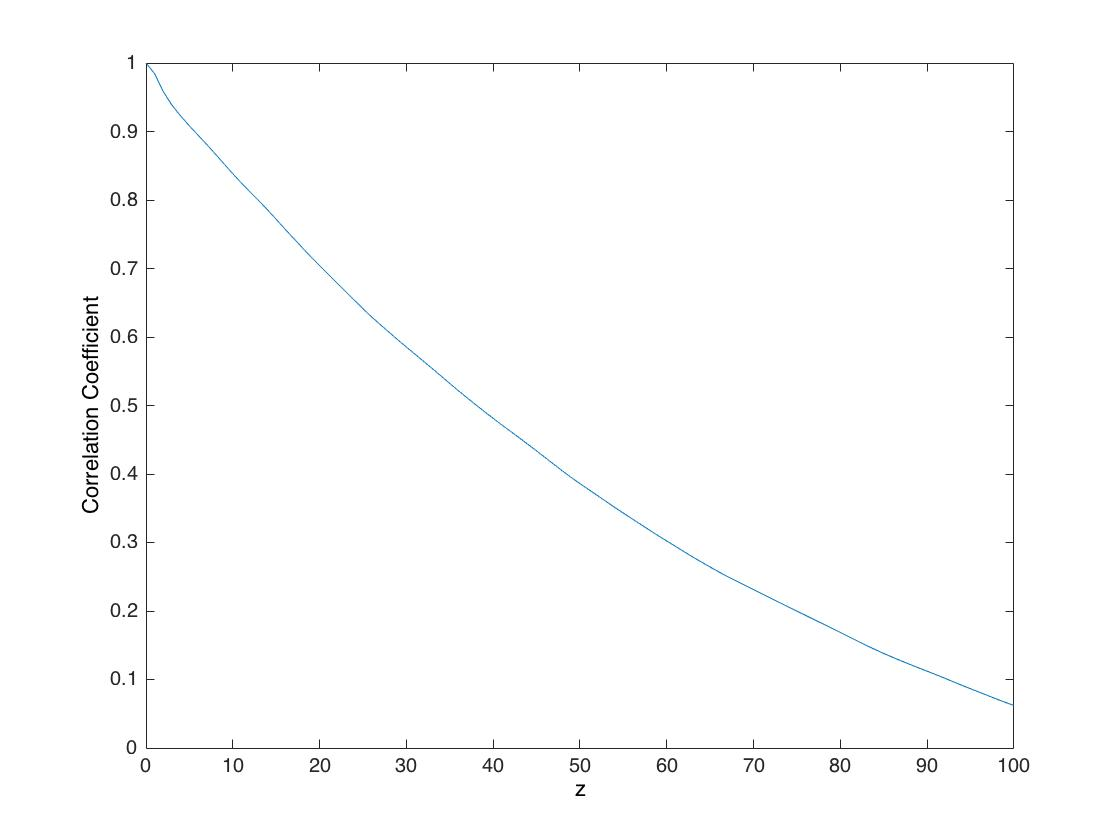
\includegraphics[width=\linewidth]{graph2.jpg}
  \caption{Task 7b}
  \label{fig:task7b}
\end{figure}

Correlation coefficient decreases as z increases. This is because when z is small the pixels are closeby and the intensity usually varies

\pagebreak


\end{document}